\section{Customized Empirical Potential and GCMC Simulation Setup for Deposition}

\begingroup
\begin{figure}[!ht]
  \centering
  \subfigure{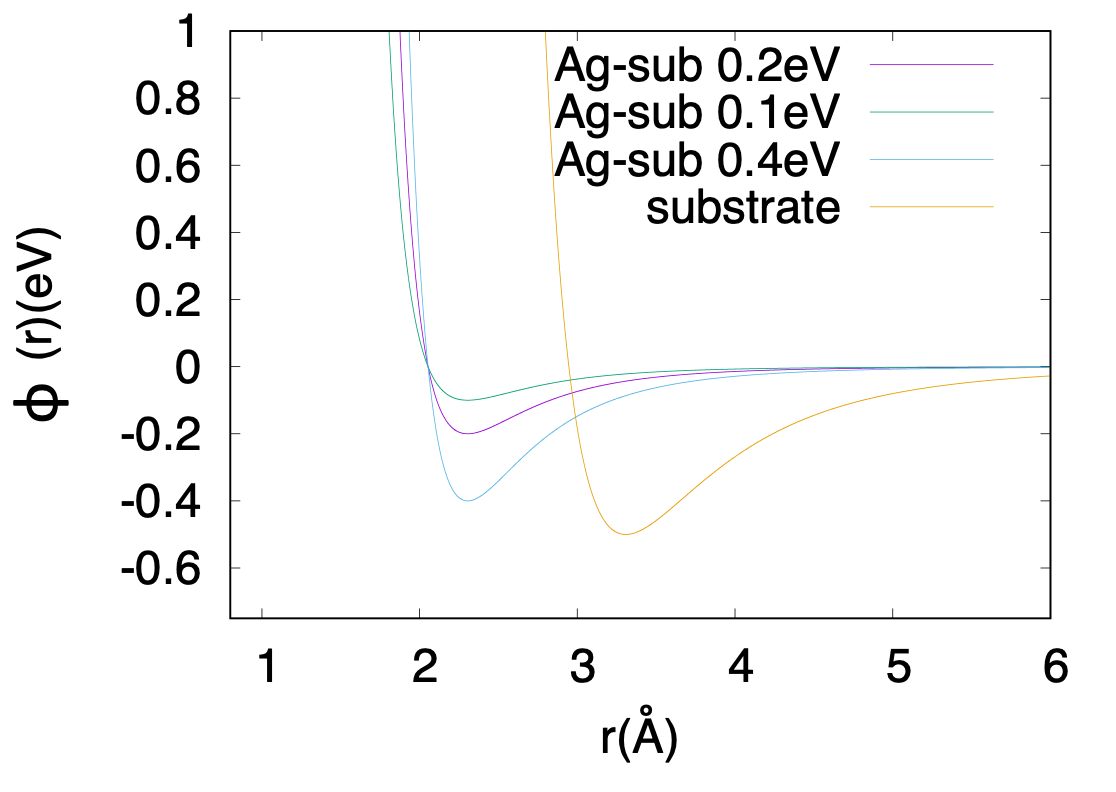
\includegraphics[width=0.8\linewidth]{Chap4/plots/Picture2.png}}
  \caption[Lennard-Jones potential used to describe different bonding strength and bond length of Ag-substrate atoms, and substrate-substrate atoms]{\ac{L-J} potential used to describe different bonding strength and bond length of Ag-substrate atoms, and substrate-substrate atoms.}
  \label{Chap:Ag/ZnO:fig2}
\end{figure}
\endgroup

In order to conduct \ac{GCMC} simulations accurately for metal deposition, a reasonable potential must be used to describe the interaction between Ag adsorbates and substrate atoms. An \ac{EAM} potential \cite{williams2016modeling} is used to describe the interaction between Ag-Ag atoms, while the interactions between Ag and substrate atoms need to be able to tune for different bonding environments. As a result, we applied simple \ac{L-J} 12-6 potential \cite{jones1924determination} for Ag-substrate interaction and interactions between substrate-substrate atoms:
\begin{align}
 \Phi_{LJ} = 4\epsilon \left[ (\frac{\sigma}{r})^{12} - (\frac{\sigma}{r})^6\right]
 \label{Chap:Ag/ZnO:eq:LJ}
\end{align}
where $\epsilon$ controls bonding strength and $\sigma$ changes equilibrium bond lengths. As shown in Figure \ref{Chap:Ag/ZnO:fig2}, purple, green and blue lines describes the interaction between Ag atom and normal, week, and strong bonding with substrates, respectively. And the equilibrium bond length is fitted for the bond distance between Ag and ZnO substrates at $\sim$ 2.3$\angstrom$. And the yellow line corresponding to the substrate interactions itself, we set the bond length based on ZnO substrates lattice constant. And a strong potential well is used in order to simulate a more rigid substrate. The \ac{GCMC} code we used is from J. Li's Group in MIT\cite{sina2017mapp}.

As we previously discussed in Chapter \ref{Chap:Mech:GCMC:GCMC}, the chemical potentials of elements of interest are used to decide the probability of accepting/rejecting a certain event. The Ag gas phase chemical potential is used, via:
\begin{align}
 \mu_{Ag(g)} = \mu_{Ag(bulk)} + k_{B}T\ln{\frac{p}{p_0}}
 \label{Chap:Ag/ZnO:eq:mu_Ag}
\end{align}
where, $p_0$ is the Ag evaporation pressure. Usually, the vacuum pressure of a sputtering chamber is $\sim$ 1 $pa$. So a chemical potential $\mu$ of -0.6 $eV$ is used to simulate $p$=1$Pa$ Ag partial pressure at 300$K$.

\newpage
\begingroup
\begin{figure}[!ht]
  \centering
  \subfigure[]{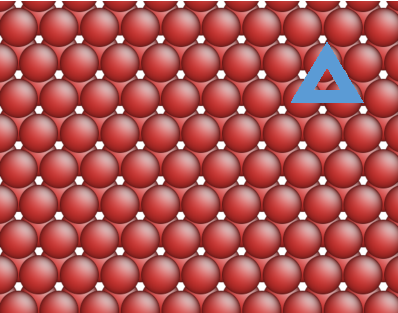
\includegraphics[width=0.45\linewidth]{Chap4/plots/Picture3a.pdf}}\label{Chap:Ag/ZnO:fig:3a}
  \subfigure[]{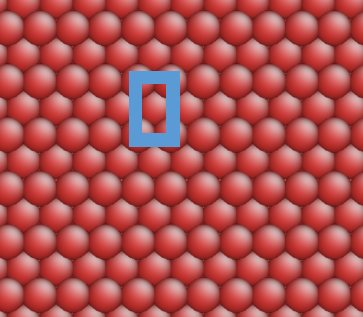
\includegraphics[width=0.40\linewidth]{Chap4/plots/Picture3b.pdf}}\label{Chap:Ag/ZnO:fig:3b}
  \\
  \subfigure[]{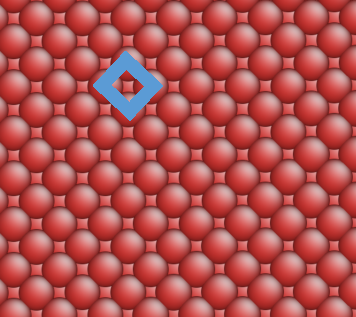
\includegraphics[width=0.42\linewidth]{Chap4/plots/Picture3c.pdf}}\label{Chap:Ag/ZnO:fig:3c}
  \subfigure[]{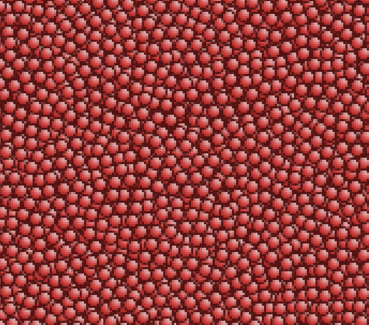
\includegraphics[width=0.42\linewidth]{Chap4/plots/Picture3d.pdf}}\label{Chap:Ag/ZnO:fig:3d}
\caption[Four different substrate types for GCMC simulation.]{Four different substrate types for GCMC simulation: (a) hexagonal, (b) rectangular, (c) square like surface lattice, and (d) amorphous surface. }
  \label{Chap:Ag/ZnO:fig3}
\end{figure}
\endgroup

Four different substrate types are used in this simulation, as shown in Figure \ref{Chap:Ag/ZnO:fig3}. Hexagonal surface unit, as shown in Figure \ref{Chap:Ag/ZnO:fig3} (a), corresponds to \ac{FCC} \{111\} surfaces and \ac{HCP} \{0001\} surfaces. Rectangular one, as shown in Figure \ref{Chap:Ag/ZnO:fig3} (b), corresponds to \ac{FCC} \{110\} surfaces and \ac{HCP} \{10$\overline{1}$0\} surfaces. Square one, as shown in Figure \ref{Chap:Ag/ZnO:fig3} (c), corresponds to \ac{FCC} \{100\} surfaces. Besides, an amorphous substrate, as shown in Figure \ref{Chap:Ag/ZnO:fig3} (d), is also created by quenching down from a high temperature. By combining different substrates with tunable \ac{L-J} potentials, different substrates with different lattice constants can be achieved. Because \ac{FCC} and \ac{HCP} structures have different ways to define lattice constant, we will use bond length in the following sections to avoid confusion. By using strong and weak bonding of Ag-substrate interactions together, one can also simulate ``anchor'' sites on a regular substrates which will be discussed in Subsection \ref{Chap:Ag/ZnO:section:anchor}.